\documentclass[11pt, letterpaper, includehead]{article}

%%%%%%%%%%%%%%%%%%%%% Pre-document %%%%%%%%%%%%%%%%%%%%%
\usepackage{fancyhdr}  % Allow for headers
\usepackage{graphicx}  % Allow for figures 
\usepackage{float}     % Allow for figure inserted in specified location
\usepackage{array}     % Allow for cell width manipulation
\usepackage{nicematrix}
\usepackage{multicol} % Multiple cols
\usepackage{tikz} % For latex graphics

\setlength{\parindent}{0pt} % Remove auto paragraph indents

% Get rid of those big ass margins
\usepackage[margin=1in]{geometry}

% Table cell formatting
\setlength{\arrayrulewidth}{0.25mm}
\setlength{\tabcolsep}{11pt}
\renewcommand{\arraystretch}{1.2}

\begin{document}

%%%%%%%%%%%%%%%%%%%%% Title Page %%%%%%%%%%%%%%%%%%%%%
\begin{titlepage}
  \begin{center}
    \Huge{\textbf{Lab 6}}\\
    \Huge{When Pigs Fly}
    \vfill
    \begin{figure}[H] % H makes the figure insert at the position in the document
      \centering
      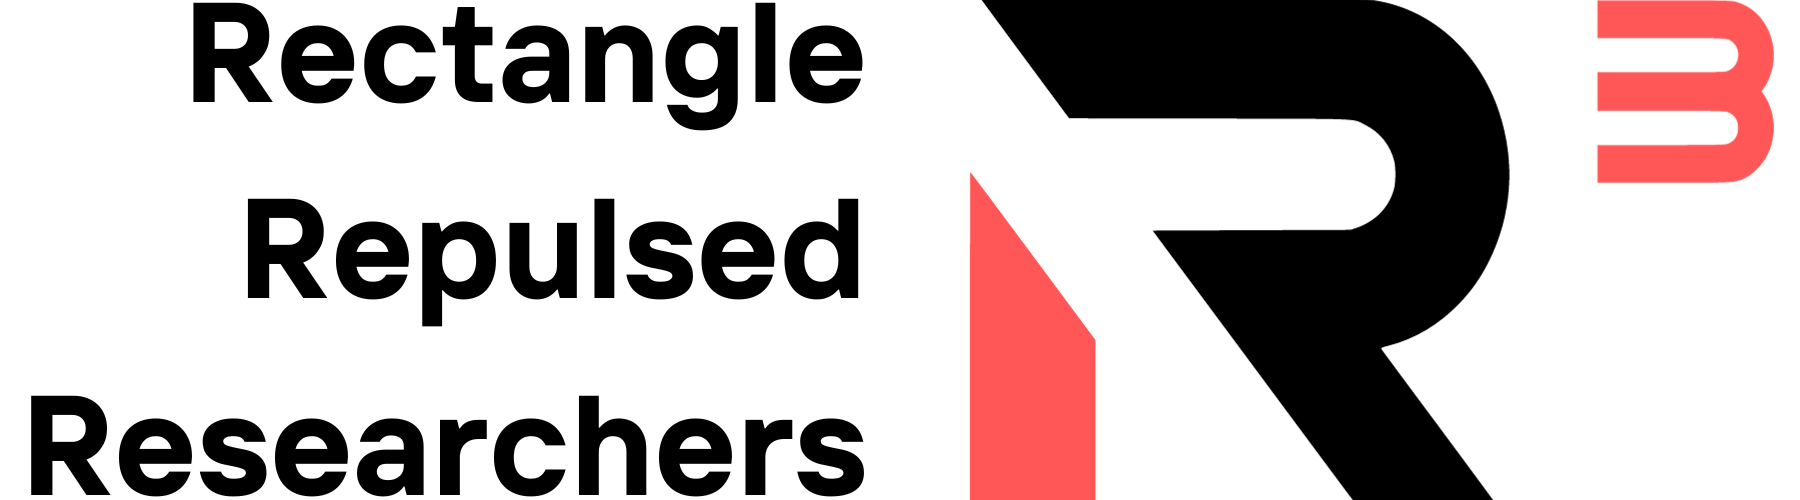
\includegraphics[width=6cm]{../logo.png}
    \end{figure}
    \large{\textbf{your name here}}\\
    \large{Julian Barossi, Liam Gilligan, Stephanie L'Heureux}\\
    \vspace{0.5cm}
    \normalsize
    \today
  \end{center}
\end{titlepage}

%%%%%%%%%%%%%%%%%%%%% TABLE OF CONTENTS %%%%%%%%%%%%%%%%%%%%%
\tableofcontents
\pagebreak % Move to next page

% Add a nice fancy header
\pagestyle{fancy}
\fancyhead{}
\fancyhead[C]{\textbf{Lab 5:} Forces and Acceleration}

%%%%%%%%%%%%%%%%%%%%%%%% SECTION 1 %%%%%%%%%%%%%%%%%%%%%%%%

\section{Set Up and Data Taking}


\subsection{Measured values}
\begin{center}
  \begin{tabular}{|  m{4cm} | m{5cm} | m{3cm} | }
    \hline
    \textbf{Quantity} & \textbf{Starting units} & \textbf{SI units} \\
    \hline
    Mass  (m)  & $110.5g\left( \frac{1kg}{10^3g}\right)$ & 0.1105 kg  \\
    \hline
    Diameter ($\Delta x$) & $1in\left( \frac{0.0254m}{1in}\right)$ & 0.0254 m  \\
    \hline
    Radius (r) & $48.25 cm \left( \frac{1m}{10^2cm}\right)$ & 0.4825 m  \\
    \hline
  \end{tabular}
\end{center}

% % Mass 
% $$m = 110.5g\left( \frac{1kg}{10^3g}\right) = 0.1105 kg $$
% % Diameter
% $$diameter = 1in\left( \frac{0.0254m}{1in}\right) = 0.0254 m$$
% % Radius
% $$r = 48.25 cm \left( \frac{1m}{10^2cm}\right) = 0.4825 m$$

\section{Analyzing the Data}
\subsection{Absolute value of the force}
\begin{center}
  \begin{tikzpicture}
    \draw[thin,dashed][->] (-2,0) -- (2,0) node[right] {$x$}; % x axis
    \draw[thin,dashed][<-] (0,-2) -- (0,2) node[above] {$y$}; % y axis
    \draw[very thick, blue][->]  (0,0) --  node [right, pos=1, color=black] {$T$} (0,1.5); % tension
    \draw[very thick, blue][->]  (0,0) -- node [right, pos=1, color=black] {$mg$} (0,-1.5); % weight
    \draw[fill=black] (0,0) circle (0.08); % point in the center
  \end{tikzpicture}
\end{center}
The tension $T$ was found to be $1.08N$ using the force sensor.

\subsection{Centripetal force from measured tension}
% Add ar pointing upward
\begin{center}
  \begin{tikzpicture}
    \draw[thin,dashed][->] (-2,0) -- (2,0) node[right] {$x$}; % x axis
    \draw[thin,dashed][<-] (0,-2) -- (0,2) node[above] {$y$}; % y axis
    \draw[very thick, blue][->]  (0,0) --  node [right, pos=1, color=black] {$T$} (0,1.5); % tension
    \draw[very thick, blue][->]  (0,0) -- node [right, pos=1, color=black] {$mg$} (0,-1); % weight
    \draw[fill=black] (0,0) circle (0.08); % point in the center
  \end{tikzpicture}
\end{center}

$$\sum F_r = T - mg$$
$$\sum F_r = (1.28136N) - (0.1105 kg)(9.8 m/s^2)$$
$$\sum F_r = 0.19840 N$$

\subsection{Speed at the lowest point}
% insert table here
$$v = \frac{\Delta x}{t}$$
$$v = \frac{0.0254 m}{0.0265139s}$$
$$v = 0.9579880742...m/s \approx 0.958 m/s$$
$$\boxed{v = 0.958 m/s}$$

\subsection{Centripetal force from measured times}
\subsubsection{Calculations}
$$\sum F_r = ma_r$$
$$\sum F_r = (m)\left( \frac{v^2}{r}\right)$$
$$\sum F_r = (0.1105 kg)\left( \frac{(0.9579880742m/s)^2}{0.4825 m}\right)$$
\subsubsection{Percent difference}
$$\%diff = \frac{|A - B|}{(A + B)/2}$$
$$\%diff = \frac{|A - B|}{(A + B)/2}$$


\section{When pigs fly}

\subsection{Free body diagram}
\begin{multicols}{2}
  \centering
  \begin{tikzpicture}
    \draw[thin,dashed][->] (-2,0) -- (2,0) node[right] {$x$}; % x axis
    \draw[thin,dashed][->] (0,-2) -- (0,2) node[above] {$y$}; % y axis
    \draw[very thick, blue][->]  (0,0) --  node [right, pos=1, color=black] {$T$} (1.5,1.5); % tension
    \draw[very thick, blue][->]  (0,0) -- node [right, pos=1, color=black] {$mg$} (0,-1.5); % weight
    \draw[fill=black] (0,0) circle (0.08); % point in the center
    \draw (0,0.5) node[right] {$\theta$}; % point in the center
    % \draw (0,0) ++(0:2) arc (0:45:2); % point in the center
    % \draw[blue] (0,0) arc[start angle=-45, end angle=90, radius=1];
  \end{tikzpicture}

  \columnbreak

  \begin{tikzpicture}
    \draw[thin,dashed][->] (-2,0) -- (2,0) node[right] {$x$}; % x axis
    \draw[thin,dashed][->] (0,-2) -- (0,2) node[above] {$y$}; % y axis
    \draw[very thick, blue][->]  (0,0) --  node [below, pos=1, color=black] {$T\sin(\theta)$} (1,0); % tension
    \draw[very thick, blue][->]  (0,0) --  node [right, pos=1, color=black] {$T\cos(\theta)$} (0,1); % tension
    \draw[very thick, blue][->]  (0,0) -- node [right, pos=1, color=black] {$mg$} (0,-1.5); % weight
    \draw[fill=black] (0,0) circle (0.08);
  \end{tikzpicture}
\end{multicols}
\pagebreak
\begin{multicols}{2}
  \center{\textbf{x-axis}}
  $$\sum F_x = ma_x$$
  $$\sum F_x = m\left(\frac{v^2}{r}\right)$$
  $$T\sin(\theta) = m\left(\frac{v^2}{r}\right)$$

  \columnbreak
  \center{\textbf{y-axis}}
  $$\sum F_y = ma_y$$
  $$\sum F_y = 0$$
  $$T\cos(\theta ) = 0$$
\end{multicols}

\end{document}
